\chapter{Estado del arte y fundamentos teóricos}

Antes de empezar a escribir código, se deben entender los conceptos fundamentales que permitirán llevar a cabo este trabajo.

Lo que se intenta mejorar utilizando Dagger es el ciclo completo de CI/CD de una aplicación. Por lo tanto, es fundamental definir los conceptos de \textit{Continuous Integration} y el \textit{Continuous Delivery}. Una vez se comprenda a qué se refieren esos términos, se podrán entender los métodos y tecnologías convencionales que permiten implementar dichos procesos. Será entonces cuando se pueda introducir Dagger, un método innovador para realizar \textit{pipelines}, el cual aporta muchas ventajas y se comparará con otras tecnologías disponibles en el sector.

\section{CI/CD}

CI/CD son las siglas de \textit{Continuous Integration}/\textit{Continuous Delivery}, o en casos más específicos, este último también se puedo conocer como \textit{Continuous Deployment}.

Se trata de un conjunto de pasos automatizados, utilizados en el desarrollo de software para llevar el código desde su implementación inicial hasta el despliegue de la aplicación. Estos pasos incluyen:

\begin{itemize}
  \item Integración de cambios en el código.
  \item La compilación de la aplicación con los cambios realizados.
  \item Realización de pruebas.
  \item Creación y publicación de imágenes de Docker y paquetes NPM.
  \item Despliegue de la aplicación (modelo \textit{push}\cite{push})
\end{itemize}

\subsection*{\textit{Continuous Integration}}

Se basa en la integración de código de manera constante, día a día, en un repositorio compartido por programadores. Cada uno de los programadores realiza cambios en el código y lo integra en el repositorio. Una vez se realizan cambios, estos deben pasar una serie de pruebas para que se incluyan definitivamente en el código fuente de la aplicación (Fig. \ref{ci}).

\begin{figure}
  \centerline{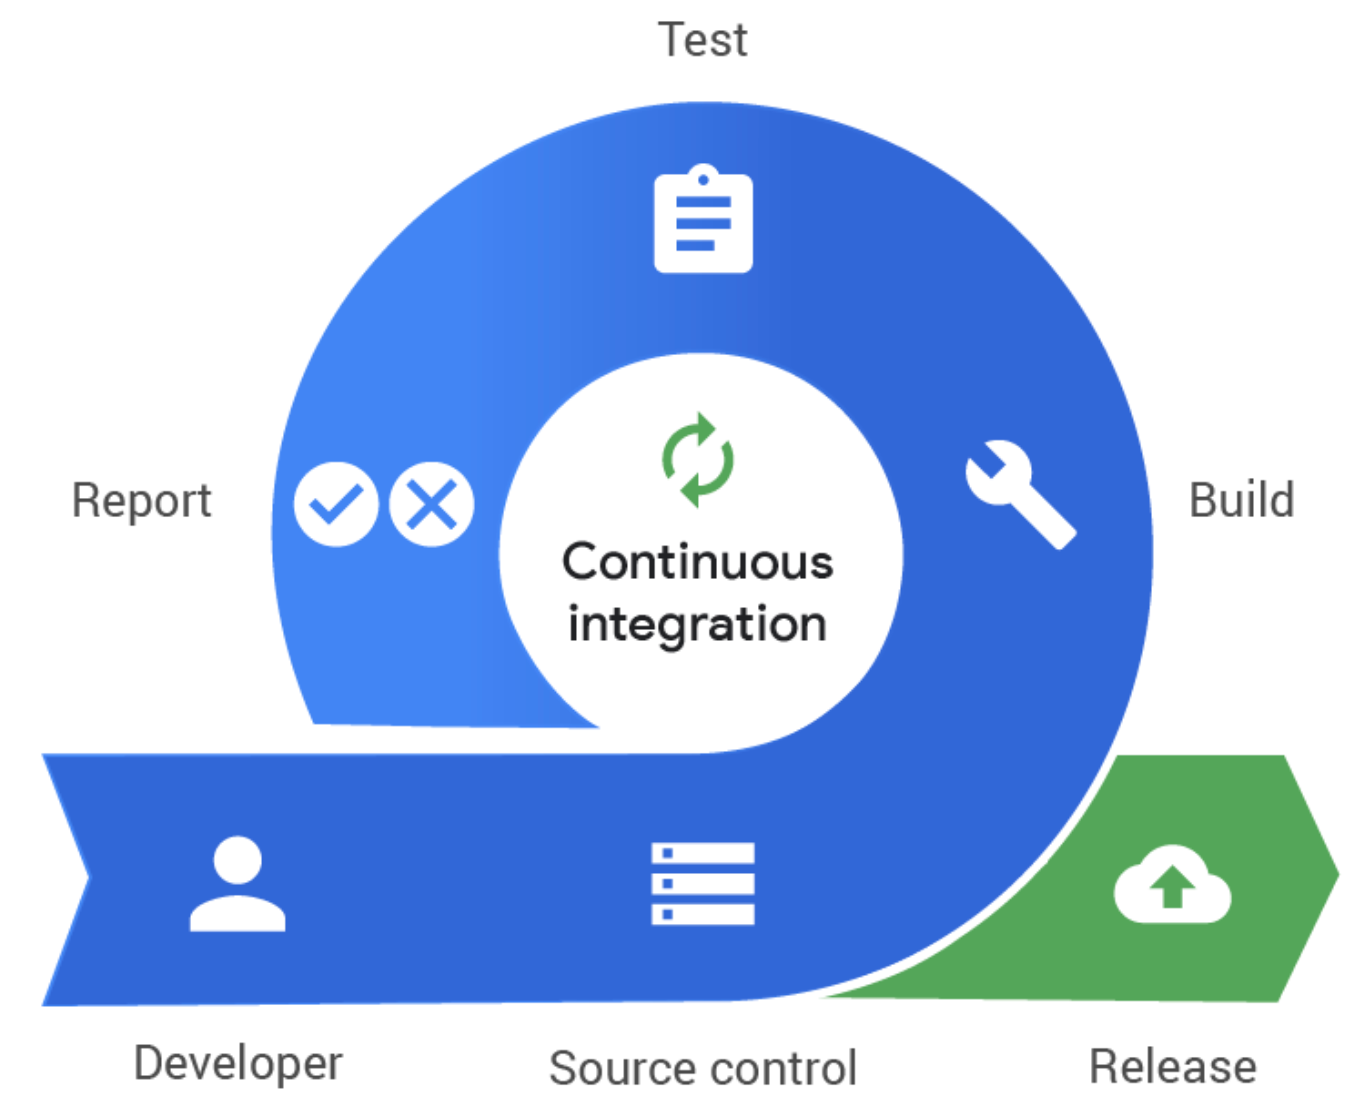
\includegraphics[width=15cm]{figuras/ci}}
  \caption{Proceso de integración continua.\cite{img.ci}}
  \label{ci}
\end{figure}


\section{Métodos convencionales}

\section{Dagger}
